\section*{三、结果与分析}

\subsection*{1. 自组电桥测量结果}

\subsubsection*{1.1 比率臂绝对值对灵敏度的影响}

按教材定义
\begin{equation}
  S=\frac{\Delta d}{\Delta R_s/R_s}
  =\frac{\Delta dR_s}{\Delta R_s}.
\end{equation}
计算得到：

\begin{table}[H]
  \centering
  \small
  \caption{比率臂绝对值与电桥灵敏度}
  \begin{tabular}{cccc}
    \toprule
    $R_1=R_2\,/\Omega$ & $\Delta d$/格 & $\Delta R_s/\Omega$ & $S$ \\
    \midrule
    30.0 & 9.0 & 0.1 & 20691 \\
    300.0 & 7.0 & 0.1 & 16072 \\
    3000 & 1.2 & 0.1 & 2753 \\
    \bottomrule
  \end{tabular}
\end{table}

第二组手写值有误。按 $R_s=229.6\ \Omega$、$\Delta d=7.0$ 格和 $\Delta R_s=0.1\ \Omega$ 重新计算，得到 $S=16072$，报告采用该重算值。

三组数据的桥臂比率均为 1，只有比率臂绝对值不同。随着 $R_1=R_2$ 从 $30.0\ \Omega$ 增大到 $3000\ \Omega$，灵敏度由 20691 降至 2753。因此，在本实验电源、检流计及待测电阻条件下，较小的比率臂绝对值可获得更高的电桥灵敏度。这三组数据用于说明灵敏度变化，不应取平均作为 $R_x$ 的重复测量结果。

因此，后续交换法测量选用灵敏度最高的 $R_1=R_2=30.0\ \Omega$ 组。

\subsubsection*{1.2 交换法测量待测电阻}

对各组数据按
\begin{equation}
  R_x=\sqrt{R_sR_s'}
\end{equation}
重新计算。第 1 组例如
\begin{equation}
  R_x=\sqrt{229.9\times230.1}\ \Omega
  =230.0\ \Omega.
\end{equation}
不同桥臂比率下的结果见表。$k=1$ 仅列上一节选定的高灵敏度代表组。

\begin{table}[H]
  \centering
  \small
  \caption{不同桥臂比率下的交换法结果}
  \begin{tabular}{ccccc}
    \toprule
    $k$ & $R_s/\Omega$ & $R_s'/\Omega$ & $R_x/\Omega$ & 相对第 1 组偏差 \\
    \midrule
    1  & 229.9 & 230.1 & 230.0 & 0 \\
    2  & 114.7 & 457.1 & 229.0 & $-0.4458\%$ \\
    3  & 76.20 & 685.4 & 228.5 & $-0.6377\%$ \\
    10 & 23.00 & 2283.2 & 229.2 & $-0.3659\%$ \\
    \bottomrule
  \end{tabular}
\end{table}

四组结果均在约 $228.5\text{--}230.0\ \Omega$ 范围内。$k=1$ 时标准电阻与待测电阻同数量级，电阻箱有效数字利用较充分，因此选取该组作为最终结果。

\subsubsection*{1.3 待测电阻的不确定度}

教材实验 4.2 对自组电桥给出的相对不确定度为
\begin{equation}
  E=\frac{\Delta R_x}{R_x}
  =\sqrt{\left(0.001+\frac{0.002m}{R_s}\right)^2
  +\left(\frac{0.2}{S}\right)^2}.
\end{equation}
六旋钮电阻箱取 $m=6$。对灵敏度最高的 $R_1=R_2=30.0\ \Omega$ 组，有
\begin{align}
  E
  &=\sqrt{\left(0.001+\frac{0.002\times6}{229.9}\right)^2
  +\left(\frac{0.2}{20691}\right)^2} \\
  &=1.052\times10^{-3}=0.1052\%,\\
  \Delta R_x&=ER_x=0.2420\ \Omega.
\end{align}
不确定度首位为 2，保留两位有效数字，并使测量值末位与不确定度末位对齐，结果为：
\begin{equation}
  \boxed{R_x=(230.00\pm0.24)\ \Omega},
  \qquad \boxed{E=0.11\%}.
\end{equation}

\subsection*{2. Cu50 温度系数}

\subsubsection*{2.1 各温度点计算}

教材给出
\begin{equation}
  \alpha_i=\frac{4U_i}{t_i(\mathcal E-2U_i)},
  \qquad \mathcal E=1.3\ \mathrm V.
\end{equation}
同时可计算
\begin{equation}
  \Delta R_i=50\alpha_it_i,
  \qquad R_{t,i}=50+\Delta R_i.
\end{equation}
例如第 1 组
\begin{equation}
  \alpha_1
  =\frac{4\times0.0335}{25.0(1.3-2\times0.0335)}
  =0.004347\ {}^\circ\mathrm C^{-1}.
\end{equation}
各组结果为：

\begin{table}[H]
  \centering
  \footnotesize
  \caption{Cu50 各温度点的计算结果}
  \begin{tabular}{ccccc}
    \toprule
    $t/{}^\circ\mathrm C$ & $U/\mathrm{mV}$ & $\Delta R/\Omega$ & $R_t/\Omega$ & $\alpha/({}^\circ\mathrm C^{-1})$ \\
    \midrule
    25.0 & 33.5 & 5.434 & 55.43 & 0.004347 \\
    30.0 & 39.6 & 6.488 & 56.49 & 0.004325 \\
    35.1 & 45.3 & 7.491 & 57.49 & 0.004269 \\
    40.0 & 51.1 & 8.532 & 58.53 & 0.004266 \\
    45.0 & 56.8 & 9.575 & 59.58 & 0.004256 \\
    50.0 & 62.7 & 10.68 & 60.68 & 0.004270 \\
    55.1 & 68.3 & 11.74 & 61.74 & 0.004262 \\
    60.1 & 74.2 & 12.89 & 62.89 & 0.004288 \\
    \bottomrule
  \end{tabular}
\end{table}

平均温度系数为
\begin{equation}
  \bar\alpha=\frac{1}{8}\sum_{i=1}^{8}\alpha_i
  =0.004285\ {}^\circ\mathrm C^{-1}.
\end{equation}
教材附录给出 Cu50 的理论值 $\alpha_0=0.004280\ {}^\circ\mathrm C^{-1}$，因此相对误差为
\begin{equation}
  \delta_\alpha
  =\frac{|\bar\alpha-\alpha_0|}{\alpha_0}\times100\%
  =0.1258\%\approx0.13\%.
\end{equation}

\subsubsection*{2.2 $U-t$ 特性曲线}

\begin{figure}[H]
  \centering
  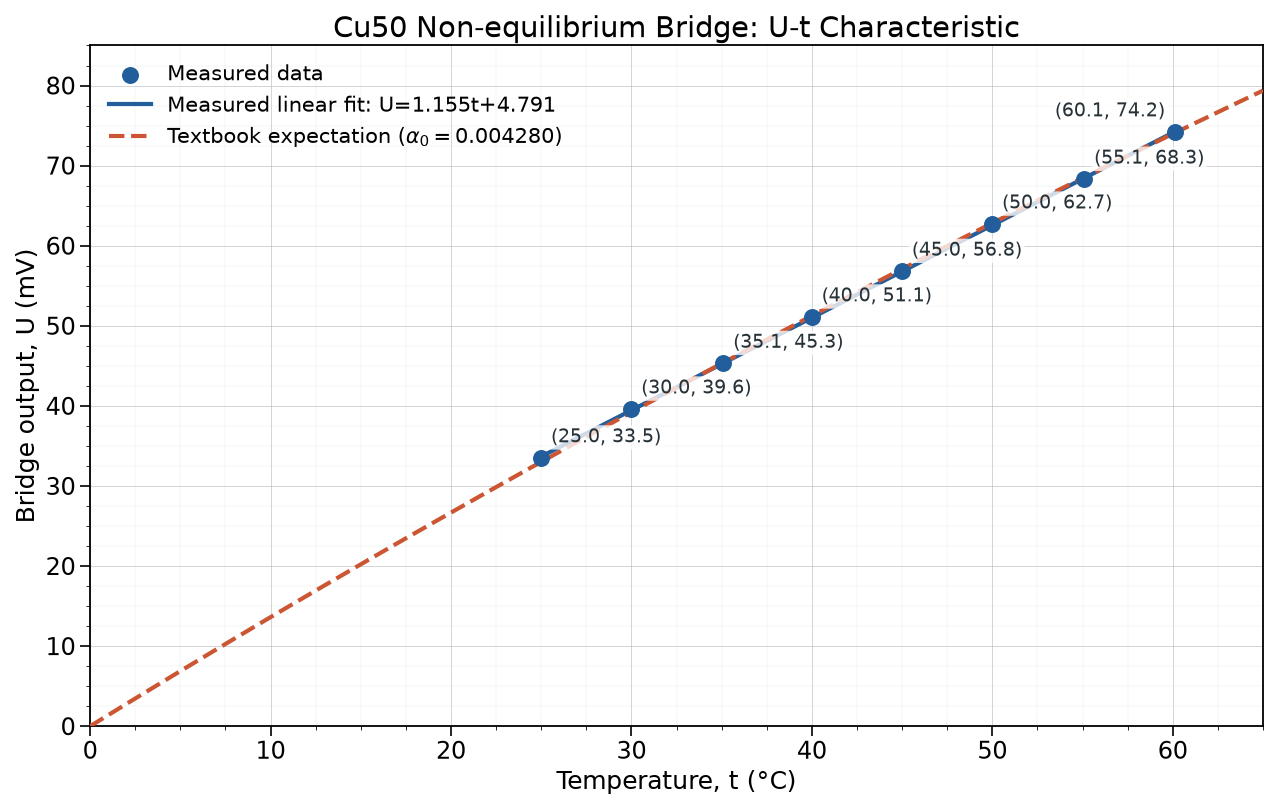
\includegraphics[width=0.82\textwidth]{assets/cu50-u-t.png}
  \caption{Cu50 非平衡电桥的 $U-t$ 特性曲线}
\end{figure}

实测数据的线性拟合为
\begin{equation}
  U/\mathrm{mV}=1.155\,t/{}^\circ\mathrm C+4.791,
  \qquad R^2=0.9999.
\end{equation}
实验点具有很好的线性趋势，并与教材理论曲线基本重合。

\subsubsection*{2.3 A 类标准不确定度}

对 8 个温度点的 $\alpha_i$ 进行统计，得
\begin{equation}
  s(\alpha)=3.318\times10^{-5}\ {}^\circ\mathrm C^{-1},
\end{equation}
\begin{equation}
  u_A(\bar\alpha)=\frac{s(\alpha)}{\sqrt8}
  =1.173\times10^{-5}\ {}^\circ\mathrm C^{-1}.
\end{equation}
按课程规则修约后
\begin{equation}
  \boxed{\bar\alpha=(4.285\pm0.012)\times10^{-3}\ {}^\circ\mathrm C^{-1}}
  \qquad (u_A,\ k=1).
\end{equation}
相对 A 类标准不确定度为 $0.274\%$。由于电压表、温度传感器和工作电源的允许误差限未知，无法评定 B 类标准不确定度，故本报告仅给出 A 类标准不确定度。

\subsection*{3. 误差分析}

\begin{enumerate}
  \item 从不同比率臂下的 $R_x$ 可以看出，测量结果在 $228.5\text{--}230.0\ \Omega$ 之间，最大值与最小值相差约 $1.5\ \Omega$。待测电阻的标称值为 $220\ \Omega$，而交换法测得 $R_x=230.0\ \Omega$，相对标称值的偏差为
  \begin{equation}
    \frac{|230.0-220|}{220}\times100\%=4.545\%\approx4.5\%.
  \end{equation}
  标称值不一定等于电阻的实际真值，而且本次实验没有记录该电阻的允许误差等级，因此不能把这 $4.5\%$ 全部看成测量误差。可能原因如下：
  \begin{itemize}
    \item \textbf{偶然误差：}调节电阻箱时，检流计指针会有轻微摆动，对“指零”位置的判断也会有少量差异；接线柱的轻微松动也可能使平衡点在重新接线后发生小幅变化。
    \item \textbf{系统误差：}比率臂和电阻箱的实际阻值与标称值可能存在偏差，导线电阻和接触电阻也会加入桥臂。交换法能减小比率臂误差的影响，但不能完全消除电阻箱示值偏差和接触电阻。
  \end{itemize}

  \item Cu50 的各组 $\alpha_i$ 在 $4.256\times10^{-3}\text{--}4.347\times10^{-3}\ {}^\circ\mathrm C^{-1}$ 之间波动，平均值为 $4.285\times10^{-3}\ {}^\circ\mathrm C^{-1}$，与教材理论值的相对误差仅为 $0.13\%$。八个实测电压与理论值的差值最小为 $-0.297\ \mathrm{mV}$，最大为 $+0.491\ \mathrm{mV}$，平均差仅为 $+0.007\ \mathrm{mV}$，未见明显的整体零点偏移。剩余偏差可能来自：
  \begin{itemize}
    \item \textbf{偶然误差：}温控仪和电压表的示数会有小幅波动；若每次读数时等待时间不完全一致，温度和电压也可能没有同时稳定，使各点计算得到的 $\alpha_i$ 产生波动。
    \item \textbf{系统误差：}计算时将电桥工作电压按标称值 $1.3\ \mathrm V$ 处理，并假定初始桥臂电阻均为 $50.0\ \Omega$。实际工作电压、桥臂电阻和 Cu50 的零度电阻若与标称值存在偏差，会使所有 $\alpha_i$ 同向变化。
  \end{itemize}

  \item 加热过程中，Cu50 传感器本身、水体和温控仪探头之间需要一定时间才能达到热平衡。若升温过快或示数刚变化就立即读数，Cu50 的实际温度会滞后于温控仪示数，从而使温度系数产生同一方向的系统偏差。所以在测量时应等待温度和电压都稳定后再同时读数。
\end{enumerate}
